\documentclass{beamer}

%Packages
\usepackage[utf8]{inputenc}
\usepackage{hyperref}

% Code
\usepackage{listings}

\lstdefinestyle{ShellCmd}{
    language=bash,
    basicstyle=\small\ttfamily,
    backgroundcolor=\color{gray!10},
    linewidth=0.9\linewidth,
    breaklines=true
}
\newcommand\shellcmd[1]{\colorbox{gray!10}{\lstinline[style=ShellCmd,mathescape]`#1`}}

% Hide navigation symbols, show git
\setbeamertemplate{navigation symbols}{}
\setbeamertemplate{footline}[frame number]

\newcommand{\inote}[1]{
  {
    \begin{itemize}
      \item #1
    \end{itemize}
  }
}

% Logos
\newcommand{\logoimage}[2]{\begingroup
\setbox0=\hbox{\includegraphics[height=#2]{#1}}%
\parbox{\wd0}{\box0}\endgroup\ }

% Have a fancy git logo
\newcommand{\git}{\logoimage{imgs/git_logo}{8pt}}
\newcommand{\github}{\logoimage{imgs/github_logo}{8pt}}

%META-INFORMATION
\title{An introduction to (version control with) \logoimage{imgs/git_logo}{40px}}
\author{Tom Wiesing}
\institute{CS Club}
\date{September 6, 2015}

\begin{document}
    %TITLEPAGE
    \frame{\titlepage}
    
    \begin{frame}{Overview}
      \begin{itemize}
          \item Introduction
          \begin{itemize}
            \item What is version control?
            \item What is git? Why use it?
          \end{itemize}
          \item Getting started with git
          \begin{itemize}
            \item How does git store versions?
            \item How do I use clone, init, add, commit?
            \item How do I share content?
          \end{itemize}
          \item Going further
          \begin{itemize}
            \item Branching \& Merging
            \item Working with Remotes
            \item Other useful commands
          \end{itemize}
          \item A brief introduction to \github
          \begin{itemize}
            \item Collaborating with other people
            \item Making issues
            \item Forking repositories and making pull requests
          \end{itemize}
      \end{itemize}
    \end{frame}
    
    \begin{frame}{Introduction (1): What is version control?}
  \begin{columns}[onlytextwidth]
    \begin{column}{0.6\textwidth}
      \begin{itemize}
          \item tracks any kind of content
            \inote{e.g. websites, software, presentations}
          \item knows about different versions
          \begin{itemize}
            \item knows what was changed when
            \item can revert changes if something goes wrong
          \end{itemize}
          \item has a collaboration component
          \begin{itemize}
            \item several people can work together on the same project
            \item changes can be synced
            \item easy to see who changed what
          \end{itemize}
        \end{itemize}
    \end{column}
    \begin{column}[t]{0.4\textwidth}
      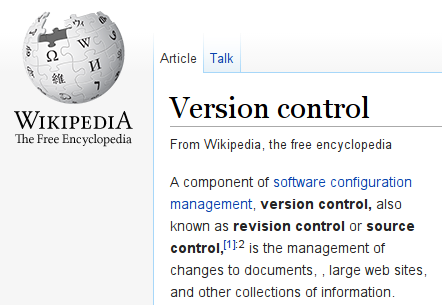
\includegraphics[width=0.95\textwidth]{imgs/vc_wikipedia}
    \end{column}
  \end{columns}
\end{frame}

\begin{frame}{Introduction (2): What is git and why use it?}
  \begin{columns}[onlytextwidth]
    \begin{column}{0.6\textwidth}
      \begin{itemize}
        \item git -- ``the stupid content tracker''
        \begin{itemize}
          \item open-source version control system
          \item fast, scalable, distributable
        \end{itemize}
        \item originally developed in 2005 for maintaining the linux kernel source code
      \end{itemize}
    \end{column}
    \begin{column}[t]{0.4\textwidth}
      
\includegraphics[width=0.95\textwidth]{imgs/git_logo}
    \end{column}
  \end{columns}
\end{frame}

\begin{frame}{Introduction (3): What is git and why use it?}
  \begin{itemize}
    \item git is both for beginners and advanced users
    \begin{itemize}
      \item provides high-level-commands
      \item additonally gives full access to internals
    \end{itemize}
    \item git is distributed - and it is easy to sync changes
    \begin{itemize}
      \item no central server to share content required
      \item changes can be synced in many ways
      \item http(s), ssh, git protocol, diffs via email, \dots
    \end{itemize}
  \end{itemize}
\end{frame}
    \begin{frame}{Getting started (1)}
  \begin{itemize}
    \item Keep in mind: This talk is only an introduction - there is more
    \item basic interaction with \git happens via the command line
    \begin{itemize}
      \item GUIs exist, but it is best to learn git from the command line
      \item Web-Frontends are widely used (we will talk about \github later)
    \end{itemize}
    \item git stores information for a single project in a \textit{git repository}
    \begin{itemize}
      \item commonly found on your hard disk in form of a folder
      \item \textit{clones} of the repository can be made in order to share it
    \end{itemize}

  \end{itemize}
\end{frame}

\begin{frame}{Getting started (2): Creating a repository}
  \begin{itemize}
    \item you can create a new repository in a folder by using \shellcmd{git init}
    \item alternatively you can clone an existing repository with \shellcmd{git clone repository-url}
    \item creates a \textit{working directory} where the current version is \textit{checked out}
    \item different versions are tracked with so-called \textit{commit}s
    \begin{itemize}
      \item has a title and some information when and by whom it was made
      \item stores a reference to the previous commit (version)
      \inote{not for the initial commit of course}
      \item stores the changes were made since that version
    \end{itemize}
  \end{itemize}
\end{frame}

\begin{frame}{Getting started (3): Working Directory, Staging Area \& History}
  \begin{columns}[onlytextwidth]
    \begin{column}{0.5\textwidth}
      \begin{itemize}
        \item commits are local to your clone - they are not automatically shared
        \item Making a commit
        \begin{itemize}
          \item first make changes in your working directory (also called the index)
          \item then add the files you want to commit to the staging area
          \item finally you commit the changes in the staging area
        \end{itemize}
      \end{itemize}
    \end{column}
    \begin{column}{0.5\textwidth}
      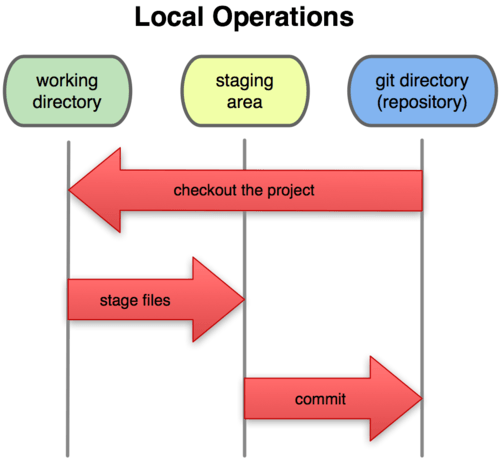
\includegraphics[width=0.95\textwidth]{imgs/git_local}
    \end{column}
  \end{columns}
\end{frame}

\begin{frame}{Getting started (4): Commands for creating commits}
  \begin{itemize}
    \item Commands for creating commits
    \begin{itemize}
      \item \shellcmd{git status} - to see what is changed and what is in the staging area
      \item \shellcmd{git add FILES} - to add files to the staging area
      \inote{use \shellcmd{git add -A .} to add everything}
      \item \shellcmd{git rm FILES} - to delete a file and add that change to the staging area
      \item \shellcmd{git commit -m MESSAGE} - to create a commit with the given message from the staging area
      \item \shellcmd{git checkout FILE} - to reset FILE to the last commit
    \end{itemize}
    \item Time for a short demo
  \end{itemize}
\end{frame}

\begin{frame}{Getting started (5): Sharing commits}
  \begin{itemize}
    \item Creating commits is great, but how to share them?
    \item git uses so called ``remotes''
    \inote{a remote is just a different clone of the same repository somewhere else}
    \item commits can be pushed to it -- using \shellcmd{git push}
    \item commits can be pulled from it -- using \shellcmd{git pull}
    \item internally it is a bit more complicated than that - we need to talk about branching first
  \end{itemize}
\end{frame}
    \begin{frame}{Going further (1): Branches}
  \begin{itemize}
    \item several people can work at the same project at the same time
    \item they might make incompatible changes (that can be united later)
    \item git allows the versions of a repository to diverge using branches
    \inote{they can also be brought back together using merging later}
    \item The default branch is usually called ``master''
    \item Each branch has a so-called HEAD that points to its latest commit
    \item There is also a HEAD of the repository which points to the current branch
  \end{itemize}
\end{frame}

\begin{frame}{Going further (2): Branching \& Merging}
  \begin{columns}[onlytextwidth]
    \begin{column}{0.5\textwidth}
      \begin{itemize}
        \item you can make commands on branches like you would normally
        \inote{but you need to switch to the branch first}
        \begin{itemize}
          \item \shellcmd{git branch name} - create a branch
          \item \shellcmd{git checkout name} - switch to it
          \item \shellcmd{git merge name} - merge a branch back into the current one
        \end{itemize}
      \end{itemize}
    \end{column}
    \begin{column}{0.5\textwidth}
      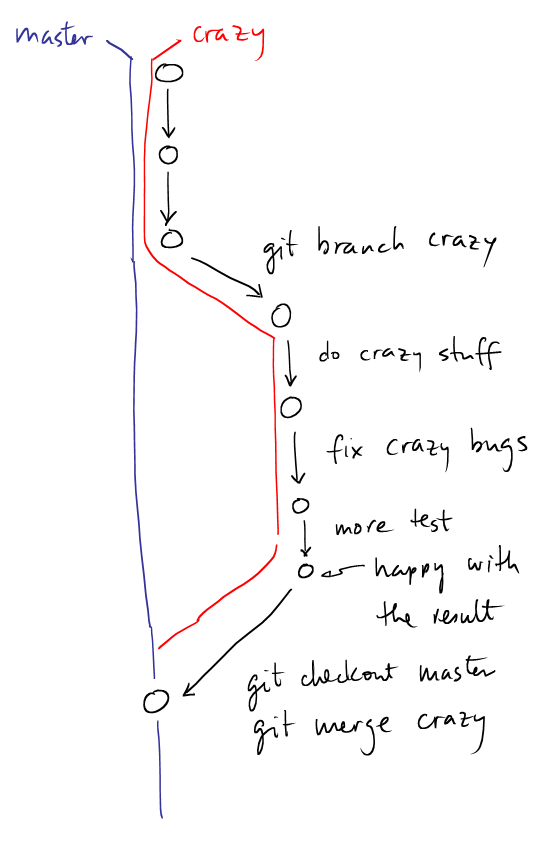
\includegraphics[height=\textheight]{imgs/branches}
    \end{column}
  \end{columns}
\end{frame}

\begin{frame}{Going further (3): Resolving Merge conflicts}
  \begin{itemize}
    \item merging can cause conflicts
    \inote{when files were modified on both branches and git can not merge them automatically}
    \item git will tell you when you run \shellcmd{git merge} if there are conflicts
    \begin{itemize}
      \item you can edit the affected files manually, then stage the files (\shellcmd{git add}) and commit them (\shellcmd{git commit})
      \inote{\shellcmd{git status} is always helpful when doing this}
      \item \shellcmd{git merge --abort} - cancel the merge and go back to what was there before
      \item ``fake'' a merge by forcing git to use one of the two versions
      \begin{itemize}
        \item \shellcmd{git merge -X ours branch} - use the version of the current branch
        \item \shellcmd{git merge -X theirs branch} - use the other branches version
        \item (you need to do this before starting to merge)
      \end{itemize}
    \end{itemize}
  \end{itemize}
\end{frame}
    \begin{frame}{A brief introduction to \github (1)}
  \begin{columns}[onlytextwidth]
    \begin{column}{0.7\textwidth}
      \begin{itemize}
        \item \github, \url{https://github.com} is a website that allows people to share and collaborate on git repositories online
          \inote{open source alternatives also exist, for example GitLab. }
        \item offers users an unlimited number of public repositories to collaborate on
        \item provides a Web Interface \& Online editor for most of gits features
        \item has a few additional features in addition to repositories
      \end{itemize}
    \end{column}
    \begin{column}{0.3\textwidth}
      
\includegraphics[width=0.9\textwidth]{imgs/Octocat}
    \end{column}
  \end{columns}
\end{frame}


\begin{frame}{A brief introduction to \github (2): Issue Tracking \& Milestones}
  \begin{itemize}
    \item Issues can be used to track bugs, todos and ideas for your project
    \item on github, anyone can comment on them
    \item people that have access to your repository can mark them as done
      \inote{This can even be done from within commit messages}
    \item you can use milestones to track your overall progress
  \end{itemize}
\end{frame}


\begin{frame}{A brief introduction to \github (3): Forking \& Pull Requests}
  \begin{itemize}
    \item sometimes you want to suggest specific changes in the code to a repository
    \item if you have access to the repository, you can just commit directly
    \item in other cases, you can ``fork'' the repository
      \inote{This makes a clone of the repository to your github account}
    \item you can then make changes in your fork and issue a pull request
    \item the owner of the original repository can then merge the changes back in
    \item time for a final demo
  \end{itemize}
\end{frame}

    \begin{frame}{The end}
      {\huge
        Thank you for your attention!\\
        Any Questions, Comments, etc?
      }
      
      \begin{itemize}
        \item Image Sources: 
        \begin{itemize}
          \item \url{https://git-scm.com/images/logos/downloads/Git-Logo-2Color.png}
          \item \url{https://git-scm.com/figures/18333fig0106-tn.png}
          \item \url{https://assets-cdn.github.com/images/modules/logos_page/GitHub-Logo.png}
          \item \url{http://www.cs.toronto.edu/~kenpu/articles/cs/git-intro/ex6.png}
          \item \url{https://en.wikipedia.org/wiki/Version_control}
          \item \url{http://cdn.meme.am/instances/500x/55168121.jpg}
          \item \url{https://assets-cdn.github.com/images/modules/logos_page/Octocat.png}
        \end{itemize}  
      \end{itemize}
    \end{frame}
\end{document}
